\chapter{CHIP8}
\label{chap:ch3}

\section{About}
\label{sec:ch3sec1}

\par CHIP8, sometimes spelled as CHIP-8, is a programming language and virtual machine specification developed by Joseph Weisbecker on the 1802 processor of the COSMAC VIP computer in the mid-1970s.

\par It was meant to be an educational tool mainly designed around creating simple video games with much more ease and less resources than conventional programming languages of the time such as BASIC.

\par Even today it is widely used as an introduction for people that are taking up software emulation as a programming hobby because of its simplicty and ease of implementation.

\vspace{1cm}

\begin{minipage}{\linewidth}
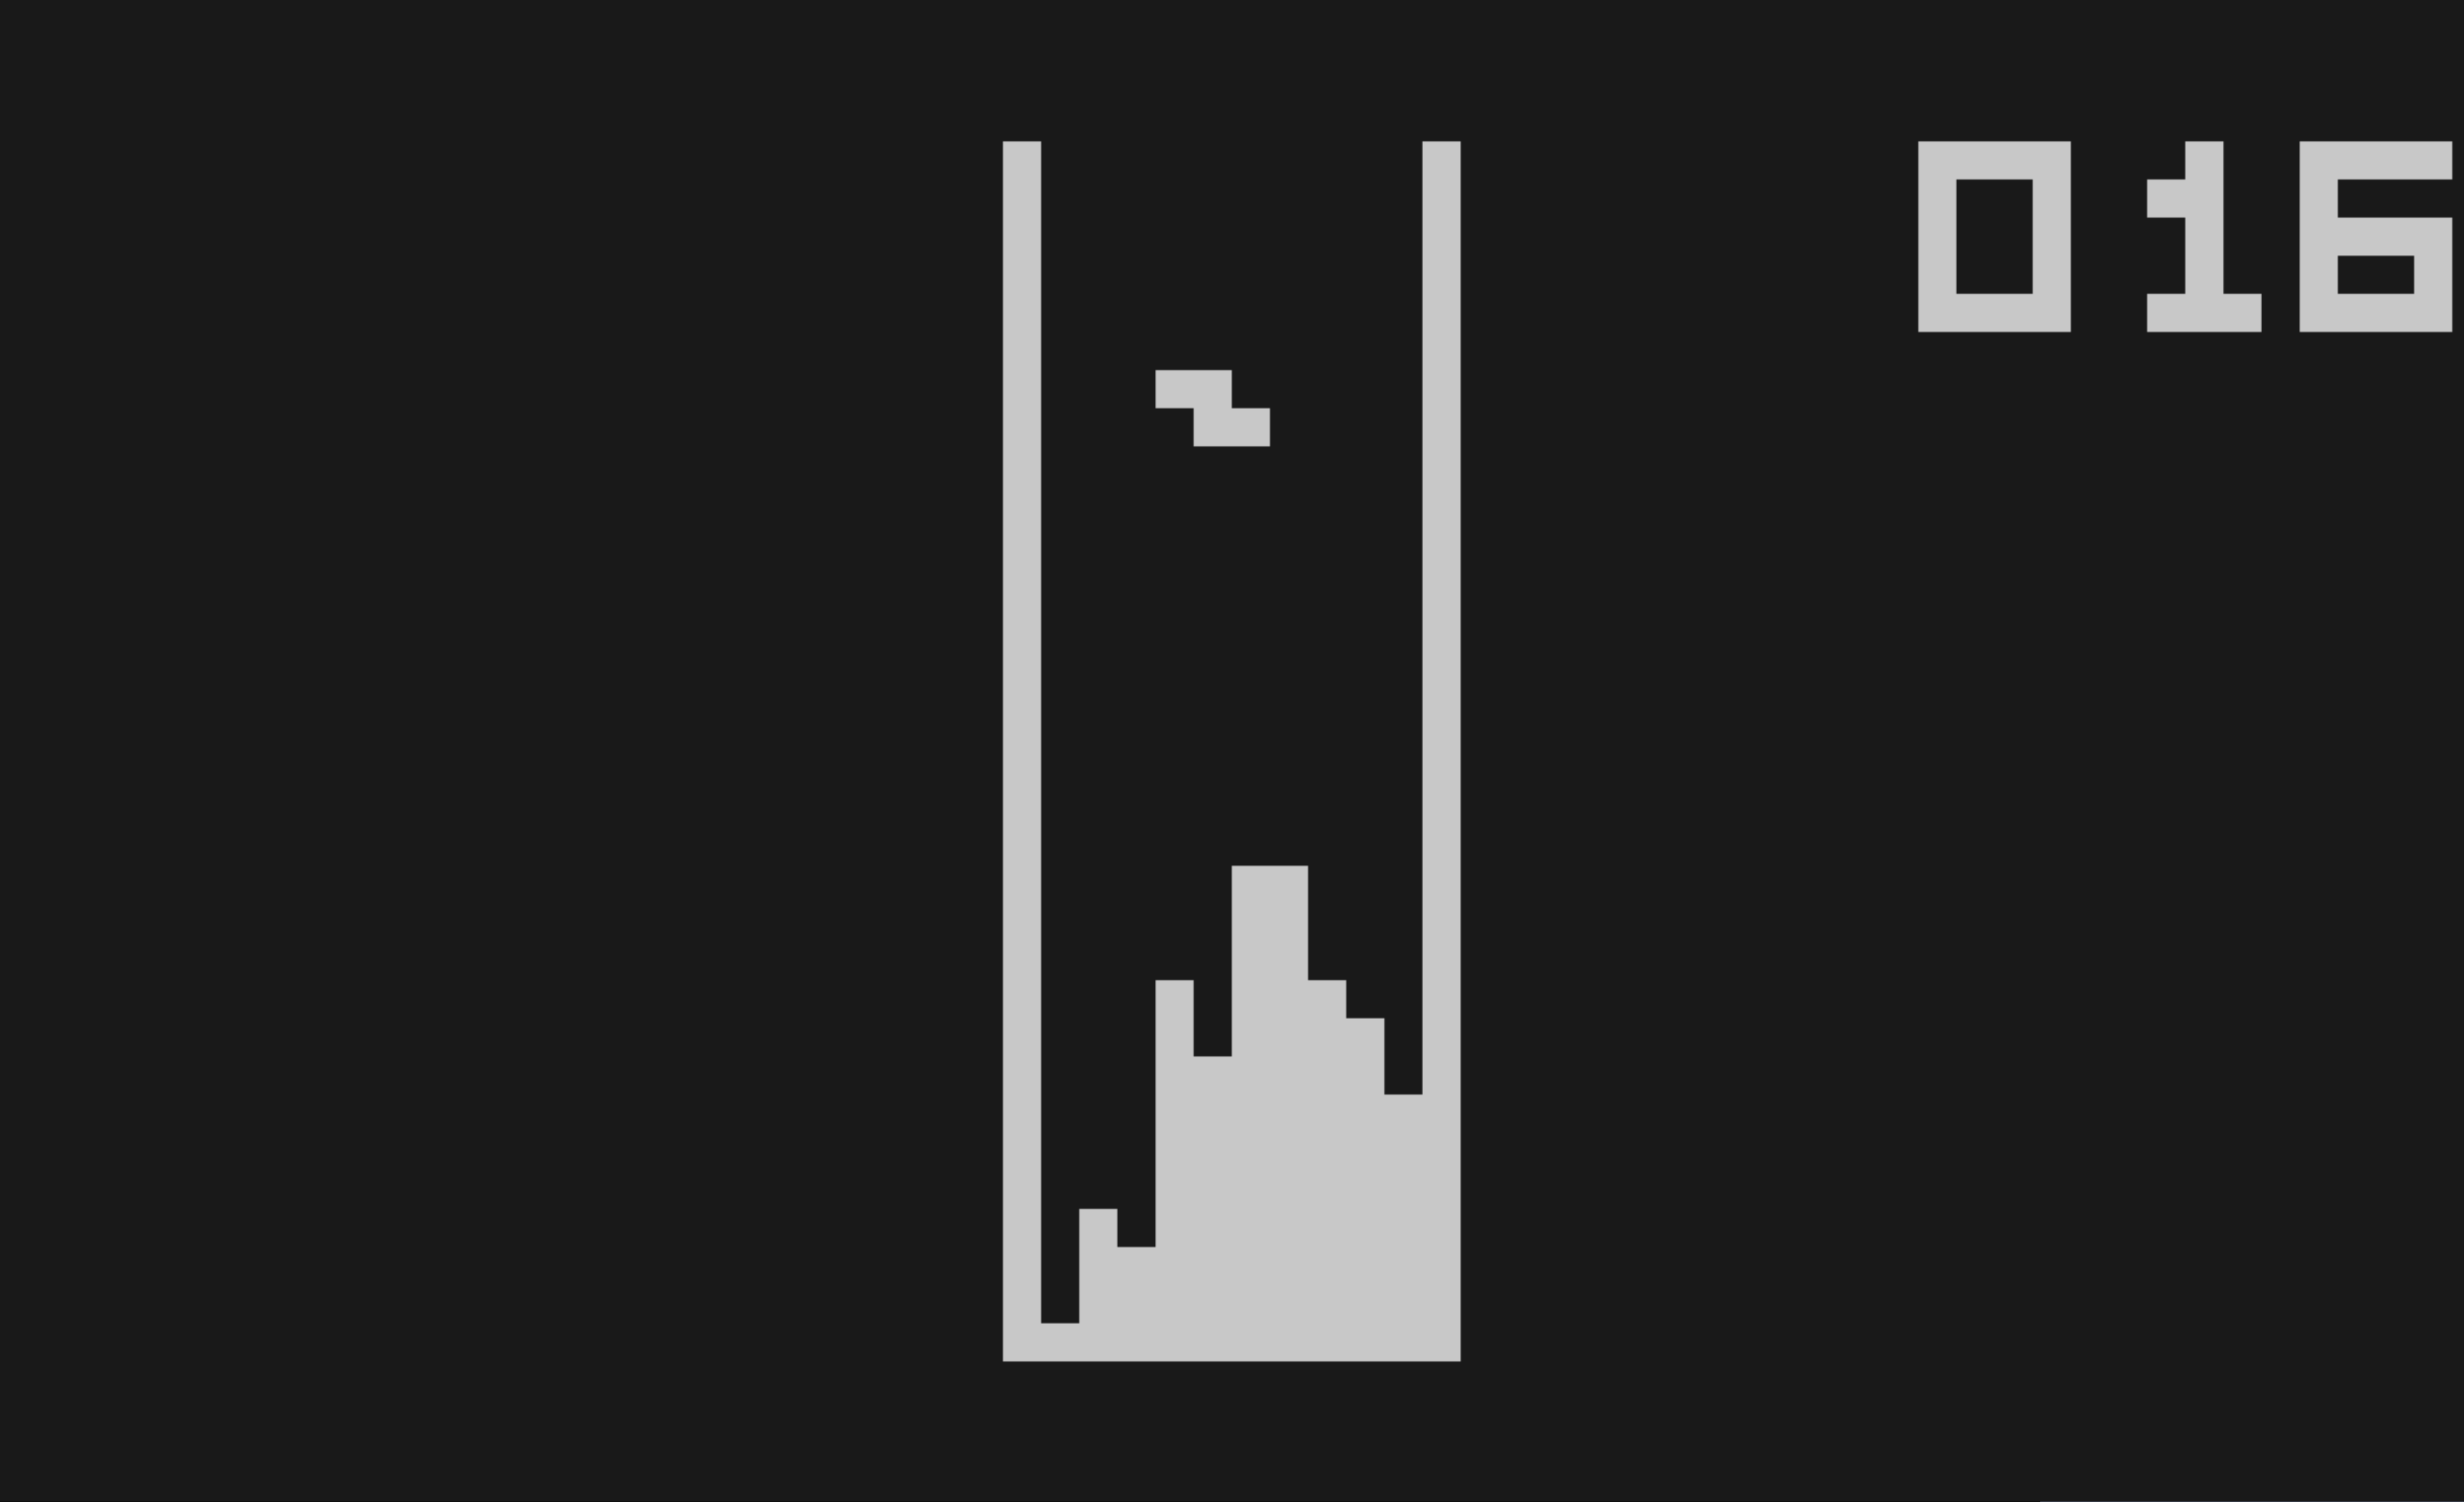
\includegraphics[width=\textwidth]{tetris_ch8}
\captionof{figure}{Tetris clone written in CHIP8 by Fran Dachille in 1991 running in \href{https://github.com/solomonarul/edra}{Edra}.}
\end{minipage}

\clearpage

\section{Virtual machine description}
\label{sec:ch3sec2}

\subsubsection{Memory}

\par The CHIP8 virtual machine has 4KB of accessible memory, as is the limit when using 16-bit memory registers. An exception occurs for the I register used mostly in drawing and array management opcodes, which is a 12-bit register instead of 16-bit. Multi-byte data is stored in big-endian format, meaning that the most significant byte of the instruction is stored first.

\par Historically, the virtual machine's space overlapped the interpreters', and as such, programs were usually loaded from address 0x200 instead. Nowadays, modern emulators use this space to store font data as they run in a separate memory space to the code they actually run. Also, the uppermost 256 bytes (addresses 0xF00-0xFFF) were used for display data and bellow that (addresses 0xEA0-0xEFF) were reserved by the interpreter for its' own internal use such as the call stack and other variables.

\subsubsection{Registers}

\par The machine also hosts 16 general use registers, adnotated V0 to VF. The register VF should not be used in normal circumstances as it is used as a flag in some operations and is also set whenever an collision occurs in the drawing of the sprites.

\subsubsection{Display}

\par The resolution of the display is 64x32 with a monochrome color. Sprites are drawn to the screen by XOR-ing themselves to the previously drawn data, where, the flag VF is set to 1 in the case of a collision (both pixels are set), like so:

\begin{table}[H]
\centering
\begin{tabular}{
>{\columncolor[HTML]{333333}}l 
>{\columncolor[HTML]{333333}}l 
>{\columncolor[HTML]{333333}}l lllll
>{\columncolor[HTML]{EFEFEF}}l 
>{\columncolor[HTML]{EFEFEF}}l 
>{\columncolor[HTML]{EFEFEF}}l l
>{\columncolor[HTML]{333333}}l l
>{\columncolor[HTML]{333333}}l }
    &                          &  &  &  &                          &  &  &  &  &  &  &  & \cellcolor[HTML]{333333} &  \\
    & \cellcolor[HTML]{EFEFEF} &  &  &  & \cellcolor[HTML]{333333} &  &  &  &  &  &  &  &                          &  \\
\cellcolor[HTML]{EFEFEF} &
    &
    \cellcolor[HTML]{EFEFEF} &
    &
    \cellcolor[HTML]{333333} &
    \cellcolor[HTML]{333333} &
    \cellcolor[HTML]{333333} &
    &
    \cellcolor[HTML]{333333} &
    \cellcolor[HTML]{333333} &
    \cellcolor[HTML]{333333} &
    &
    &
    &
    \\
    & \cellcolor[HTML]{EFEFEF} &  &  &  & \cellcolor[HTML]{333333} &  &  &  &  &  &  &  &                          &  \\
    &                          &  &  &  &                          &  &  &  &  &  &  &  & \cellcolor[HTML]{333333} & 
\end{tabular}
\caption{Illustration of sprite XOR-ing, transforming an 8 (left) into a 0 (right), VF is set in this case to 1}
\end{table}

\par The machine also has two timers, called the delay and sound timer, respectivelly. They both tick down at a rate of 60hz, and when the sound timer is non-zero, a sound is played. The specifics of the sound are not specifically defined, so it is left up to the developer of the emulator to implement however they want, the most preffered way of implementing it is by making it be a buzzer.

\clearpage

\subsubsection{Input}

\par Input is done with a 16-key keyboard, with keys having values from 0 to F, an usual input mapping to modern hardware being done like so:

\begin{table}[H]
\centering
\begin{tabular}{| c | c | c | c |}
\hline
1 & 2 & 3 & C \\ \hline
4 & 5 & 6 & D \\ \hline
7 & 8 & 9 & E \\ \hline
A & 0 & B & F \\ \hline
\end{tabular}
\caption{Original input layout on the COSMAC VIP}
\end{table}

\begin{table}[H]
\centering
\begin{tabular}{| c | c | c | c |}
\hline
1 & 2 & 3 & 4 \\ \hline
Q & W & E & R \\ \hline
A & S & D & F \\ \hline
Z & X & C & V \\ \hline
\end{tabular}
\caption{Commonly used layout on modern keyboards}
\end{table}

\subsubsection{Instructions}

\begin{longtable}{|c|c|p{9cm}|}
\hline
\textbf{Opcode} & \textbf{Mnemonic} & \textbf{Description} \\
\hline
\endfirsthead

\hline
\textbf{Opcode} & \textbf{Mnemonic} & \textbf{Description} \\
\hline
\endhead

\hline
\endfoot

\hline
\endlastfoot

00E0 & CLS & Clear the display. \\
00EE & RET & Return from a subroutine. \\
1NNN & JP addr & Jump to location NNN. \\
2NNN & CALL addr & Call subroutine at NNN. \\
3XNN & SE Vx, byte & Skip next instruction if Vx is equal to NN. \\
4XNN & SNE Vx, byte & Skip next instruction if Vx is not equal to NN. \\
5XY0 & SE Vx, Vy & Skip next instruction if Vx is equal to Vy. \\
6XNN & LD Vx, byte & Set Vx = NN. \\
7XNN & ADD Vx, byte & Set Vx = Vx + NN. \\
8XY0 & LD Vx, Vy & Set Vx = Vy. \\
8XY1 & OR Vx, Vy & Set Vx = Vx OR Vy. \\
8XY2 & AND Vx, Vy & Set Vx = Vx AND Vy. \\
8XY3 & XOR Vx, Vy & Set Vx = Vx XOR Vy. \\
8XY4 & ADD Vx, Vy & Set Vx = Vx + Vy, set VF = carry. \\
8XY5 & SUB Vx, Vy & Set Vx = Vx - Vy, set VF = NOT borrow. \\
8XY6 & SHR Vx {, Vy} & Set Vx = Vx SHR 1. \\
8XY7 & SUBN Vx, Vy & Set Vx = Vy - Vx, set VF = NOT borrow. \\
8XYE & SHL Vx {, Vy} & Set Vx = Vx SHL 1. \\
9XY0 & SNE Vx, Vy & Skip next instruction if Vx is not equal to Vy. \\
ANNN & LD I, addr & Set I = NNN. \\
BNNN & JP V0, addr & Jump to location NNN + V0. \\
CXNN & RND Vx, byte & Set Vx = random byte AND NN. \\
DXYN & DRW Vx, Vy, nibble & Display n-byte sprite starting at memory location I at (Vx, Vy), set VF = collision. \\
EX9E & SKP Vx & Skip next instruction if key with the value of Vx is pressed. \\
EXA1 & SKNP Vx & Skip next instruction if key with the value of Vx is not pressed. \\
FX07 & LD Vx, DT & Set Vx = delay timer value. \\
FX0A & LD Vx, K & Wait for a key press, store the value of the key in Vx. \\
FX15 & LD DT, Vx & Set delay timer = Vx. \\
FX18 & LD ST, Vx & Set sound timer = Vx. \\
FX1E & ADD I, Vx & Set I = I + Vx. \\
FX29 & LD F, Vx & Set I = location of sprite for digit Vx. \\
FX33 & LD B, Vx & Store BCD representation of Vx in memory locations I, I+1, and I+2. \\
FX55 & LD [I], Vx & Store registers V0 through Vx in memory starting at location I. \\
FX65 & LD Vx, [I] & Read registers V0 through Vx from memory starting at location I. \\
\end{longtable}

\par The original CHIP8 implementation featured 35 instructions, of which only 31 were initially documented in the specification as opcodes 8XY3, 8XY6, 8XY7 and 8XYE were not mentioned.

\par This is probably because all of the 8000 opcodes were part of the original CPU, the 1802's Arithmetic Logic Unit and thus were not intended to be part of the instruction set as they were not part of the interpreter itself.

\par Future extensions will add and modify the way in which these functions operate, such as in the case of instruction FX55 and FX65 which modify the I register by incrementing it for each copied byte, while the SCHIP extensions does not do that.

\clearpage

\section{Emulator implementation}
\label{sec:ch3sec3}

\par The main CHIP8 library, \href{https://github.com/solomonarul/cchip8}{cchip8}, has been split in several modules: the state, the interpreter and the static compiler. Only the runners require the state, nothing else depends on eachother.

\par The state is responsible for handling the way in which the executor is supposed to communicate with the outside by storing fucntion pointers to user procedures and other miscellanious data, such as the registers.

\begin{minted}[
    linenos,                % add line numbers
    fontfamily=tt,          % typewriter font
    fontsize=\small,        % size
    breaklines,             % allow line breaks
    tabsize=4               % size of tab
]{C}
struct chip8_state
{
    bool draw_flag;
    ... mode;
    uint16_t pc, i, stack[0x100];
    uint8_t display_width, display_height;
    uint8_t v[0x10], sp, dt, st, last_key;
    uint16_t lowres_font_address, hires_font_address;
    
    // Callbacks.
    chip8_read_b_f read_b;
    chip8_read_w_f read_w;
    chip8_write_b_f write_b;
    chip8_draw_sprite_f draw_sprite;
    chip8_clear_f clear_screen;
    chip8_key_status_f get_key_status;
    chip8_random_f get_random;
    chip8_resize_f resize;
    chip8_scroll_f scroll;
    
    void* aux_arg;  // Used for passing data to the callbacks.
};
\end{minted}

\subsection{Interpreter}
\label{subsec:ch3sec3sub1}

\par Lorem ipsum dolor sit amet, consectetur adipiscing elit, sed do eiusmod tempor incididunt ut labore et dolore magna aliqua. Ut enim ad minim veniam, quis nostrud exercitation ullamco laboris nisi ut aliquip ex ea commodo consequat. Duis aute irure dolor in reprehenderit in voluptate velit esse cillum dolore eu fugiat nulla pariatur. Excepteur sint occaecat cupidatat non proident, sunt in culpa qui officia deserunt mollit anim id est laborum

\subsection{Just-in-time compiler}
\label{subsec:ch3sec3sub2}

\par Lorem ipsum dolor sit amet, consectetur adipiscing elit, sed do eiusmod tempor incididunt ut labore et dolore magna aliqua. Ut enim ad minim veniam, quis nostrud exercitation ullamco laboris nisi ut aliquip ex ea commodo consequat. Duis aute irure dolor in reprehenderit in voluptate velit esse cillum dolore eu fugiat nulla pariatur. Excepteur sint occaecat cupidatat non proident, sunt in culpa qui officia deserunt mollit anim id est laborum

\section{Quirks and extensions}
\label{sec:ch3sec4}

\subsection{Modern Super CHIP8}
\label{subsec:ch3sec4sub1}

\begin{minipage}{\linewidth}

\includegraphics[width=\textwidth]{octogon_ch8}
\captionof{figure}{Octogon by John Earnest running in \href{https://github.com/solomonarul/edra}{Edra's} modern SCHIP mode.}
\end{minipage}

\section{Testing}
\label{sec:ch3sec5}